\documentclass{bioinfo}
\copyrightyear{2007}
\pubyear{2007}

\begin{document}
\firstpage{1}

\title[Rapid and accurate peptide identification]{Rapid and accurate
  peptide identification from tandem mass spectra}
\author[Park \textit{et~al}]{Christopher Park$^{\rm a}$, Aaron Klammer$^{\rm a}$,
Lukas K\"{a}ll$^{\rm a}$, 
William S. Noble\,$^{\rm a,b,}$\footnote{To whom correspondence should be addressed}}
\address{
$^{\rm a}$Department of Computer Science and Engineering,
$^{\rm b}$Department of Genome Sciences, University of Washington,
  Seattle, WA, USA
}
\history{Received on XXXXX; revised on XXXXX; accepted on XXXXX}

\editor{Associate Editor: XXXXXXX}

\maketitle

\begin{abstract}
\section{Motivation:}  Mass spectrometry, the core technology in the
field of proteomics, promises to enable scientists to identify and
quantify the entire complement of proteins in a complex biological
sample.  Currently, the primary bottleneck in this type of experiment
is computational.  Existing algorithms for interpreting mass spectra
are slow and fail to identify a large proportion of the given spectra.

\section{Results:} We describe a database search program called Crux
that extends the state of the art in peptide identification in several
significant respects.  Crux reimplements and extends the widely used
database search program SEQUEST.  For speed, Crux uses a peptide
indexing scheme to rapidly retrieve candidate peptides for a given
spectrum.  For each peptide in the target database, Crux generates
shuffled decoy peptides on the fly, providing a good null model and,
hence, accurate false discovery rate estimates.  In a second analysis
stage, Crux trains a machine learning model to discriminate between
target and decoy peptides, thereby significantly improving the overall
rate of peptide identification.

\section{Availability:}
\href{http://noble.gs.washington.edu/proj/crux}{http://noble.gs.washington.edu/proj/crux}
\section{Contact:} \href{noble@gs.washington.edu}{noble@gs.washington.edu}
\end{abstract}

\section{Introduction}

Tandem mass spectrometry is the method of choice for many protein
identification studies.  However, this technology suffers from an
analysis bottleneck, with a need for more efficient and more accurate
methods of mapping from the observed fragmentation spectra to the
corresponding peptides.

The most widely used methods for peptide identification, such as
SEQUEST \cite{eng:approach}, MASCOT \cite{FIXME}, Tandem \cite{FIXME}
and Inspect \cite{FIXME}, exploit a database of known protein
sequences.  For each observed spectrum, these methods search the
database for the peptide whose theoretical spectrum best matches the
observed spectrum.  The resulting peptide-spectrum matches (PSMs) can
be ranked using a pre-defined score function, or by using machine
learning methods such as linear discriminant analysis
\cite{keller:empirical}, support vector machines \cite{anderson:new,
kall:semi-supervised} or decision trees \cite{elias:intensity}.

\begin{figure}
\centering
Insert figure here.
\caption{{\bf The Crux algorithm.}  Crux takes as input a collection
  of fragmentation spectra and a target protein sequence database, and
  produces a list of peptide-spectrum matches, each with an associated
  $q$-value.
  \label{figure:crux}}
\end{figure}

In this work, we describe a computational tool called Crux that solves
the peptide identification problem efficiently and accurately.  As
illustrated in Figure~\ref{figure:crux}, Crux incorporates a rapid
peptide lookup scheme, a static scoring system for relative ranking of
peptides with respect to each spectrum, a null model based on a decoy
database of shuffled peptides generated on the fly, and a dynamically
trained support vector machine for ranking the complete collection of
PSMs.  Relative to the current state of the art, Crux makes the
following primary contributions:

\begin{itemize}

\item {\bf Efficient retrieval of candidate peptides.}  Given a
  spectrum with a specified precursor mass-to-charge ratio (m/z), Crux
  uses a precomputed peptide database to retrieve efficiently all
  peptides whose m/z lies within a user-specified window around the
  target m/z (called {\em candidate peptides}).  The database is
  sorted by peptide mass and is stored on disk, with mass indices
  stored in memory.  We show that, relative to SEQUEST's strategy of
  reading the protein sequence database from disk for each new
  spectrum, the indexed database decreases search time by X\% on
  average.

\item {\bf On-the-fly generation of decoy peptides.}  In evaluating
  the statistical significance of a PSM, mass spectrometrists
  frequently employ a {\em decoy database} comprised of protein
  sequences that have been reversed, shuffled or generated from a
  Markov chain derived from the given {\em target database}.  The
  number of matches to the decoy database yields an estimate of the
  false discovery rate associated with a collection of target PSMs.
  Crux uses this target-decoy strategy, generating decoys by shuffling
  the target peptides.  This approach ensures that each decoy peptide
  exhibits precisely the same amino acid composition and total mass as
  the corresponding target decoy.  To avoid the memory overhead
  associated with storing shuffled, non-overlapping decoy peptides in
  memory, Crux generates decoy peptides on the fly.

\item {\bf Dynamically trained PSM scoring function.}  After scoring
  all peptides with respect to a given spectrum, the top-ranked PSM
  must be ranked with respect to other PSMs from the same data set.
  Some score functions, such as SEQUEST's cross-correlation score
  (XCorr), have been used to carry out both relative ranking and
  absolute rankings; however, numerous studies have demonstrated that
  better absolute rankings can be achieved by using machine learning
  methods \cite{keller:empirical, anderson:new, elias:intensity,
  kall:semi-supervised}.  Crux incorporates a recently described
  method, called Percolator, for training a machine learning method to
  discriminate between target and decoy PSMs.  This dynamically
  trained model incorporates specific characteristics of the given
  data set.  Furthermore, Crux's implementation of Percolator allows
  the user to include the observed and predicted liquid chromatography
  retention time \cite{klammer:effect} as an additional feature.

\item {\bf Accurate false discovery rate estimates.}  Crux uses
  well-established statistical methods to estimate false discovery
  rates based upon decoy PSMs \cite{benjamini:controlling}.  To avoid
  biasing the estimates, separate sets of decoy PSMs are used to train
  the machine learning method and to estimate the final false
  discovery rate.  Crux reports, along with each PSM, a $q$-value,
  which is defined as the minimal false discovery rate threshold at
  which a given PSM is deemed correct \cite{storey:statistical}.

\end{itemize}

Perhaps most significantly, from the perspective of the mass
spectrometry research community, Crux provides all of the above in a
single stand-alone C++ program which is distributed, with source code,
free for academic use.  Below, we demonstrate that Crux is both
efficient and accurate, yielding FIXME.

\section{Approach}

\subsection{Indexing}
When given a protein fasta file as input, we generate an index of all
of its peptides on disk. The database created on disk is then used
during runtime as an input to generate candidate peptides within the
mass window of the query spectrum m/z. The main difficulties in
creating a database is first, dealing with memory shortage problems
caused by the large number of peptides,second, reducing the disk size
of the database. The key strategy to resolve the memory shortage
problem was to temporary store peptides in separate bins(file handles)
divided by mass interval, then sort each bin individually. By
partitioning the peptides into different mass bins, the total amount
of peptides needed to be sorted at one instance reduces dramatically
compared to sorting all the peptides together, thus reducing the
amount of memory needed to store the peptides. Reducing the disk size
of the database was accomplished by only storing information that was
not already present in the fasta file. For instance, instead of
storing the sequence of each individual peptide, only the protein
index, the start index and the peptide length are stored, thus when
needed, the program can quickly retrieve the sequence from the
original fasta file.

\subsection{Scoring}
We re-implemented the two scoring functions Sp, Xcorr used in SEQUEST
for Crux.  First, the preliminary scoring function Sp is used to
extract the top 500 candidate peptides. To avoid erroneous scores by
noise, the spectrum is preprocessed by square rooting and smoothing
all peak intensities before extracting the top 200 abundant peaks to
be scored for Sp.  Second, The main scoring function Xcorr is used for
the final cross-correlation analysis. A similar preprocessing step
used in Sp is applied in Xcorr. For further detail on scoring function
and preprocessing steps refer to source code.

\subsection{Null peptide generation}
\subsection{Percolator}
\subsection{Parallelization}

\begin{methods}
\section{Methods}

\end{methods}

\section{Results}

\begin{figure}
  \centering
  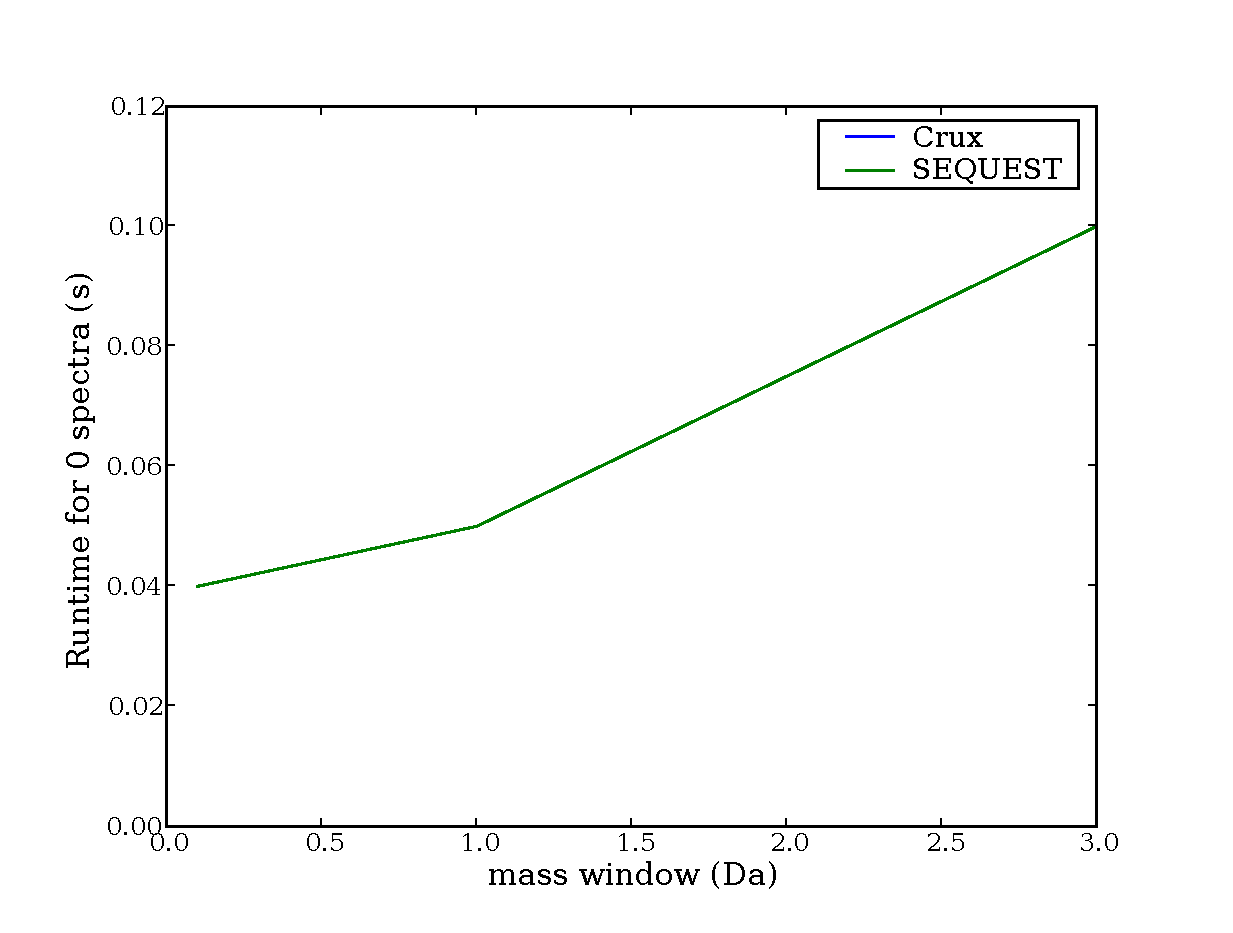
\includegraphics[width=3in]{indexing.eps}
  \caption{{\bf Rapid database searching.}  The figure plots the total
  running time required to search 10,000 tandem mass spectra against
  the non-redundant protein database, plotted as a function of the m/z
  tolerance used to define candidate peptides.  The two series
  correspond to searching with SEQUEST and searching with Crux.  For
  purposes of comparison, Crux's decoy searching and the Percolator
  post-processor are turned off.
  \label{figure:indexing}}
\end{figure}

\begin{figure*}
  \centering
  \begin{tabular}{cc}
  Insert figure here &
  Insert figure here \\
  A & B \\
  \end{tabular}
  \caption{{\bf Re-implementation of Sp and Xcorr scoring functions.}
  The figure plots, for a collection of peptide-spectrum matches, the
  Sp (panel A) and XCorr (panel B) scores as computed by Crux as a
  function of the same scores as computed by SEQUEST.
  \label{figure:indexing}}
\end{figure*}

\begin{figure}
  \centering
  Insert figure here
  \caption{Positives vs. q-value (a measure of false discovery rate) for
  standard database search algorithms, and our implementation.}
  \label{figure:indexing}
\end{figure}

Hardware: All experiments were performed on RedHat linux machine with
Athlon MP 2000, 2 x 1.67 GHz processor and 2GB of RAM.  First, using
Crux, we precomputed a peptide database for tryptic peptides of length
6 to 50 amino acids while allowing missed cleavage sites in the
nr-db(06/02/2007, 3,292,818 proteins). This procedure required 19hrs
and 14GB of disk space.

Second, we verified that our re-implemented SP and Xcorr scoring
functions are identical to the scores computed by SEQUEST.

Third, to test our indexing method for candidate peptide generation,
we compared its runtime to SEQUEST.  We use a modified version of
SEQUEST that only computes Sp (and not XCorr), and we compare its
running time to that of Crux.  For both methods, we performed searches
with 100 different spectra, using a mass tolerance of 3.  SEQUEST
required 3.55hrs clock time. Crux required 0.58hrs clock time, which
is roughly a six-fold speed improvement. We also tested Crux using a
smaller mass tolerance window, such as might be used with
high-resolution mass spectrometry instrumentation.  As the mass
tolerance window decreases, Crux's speed improves, because fewer
candidate peptides are retrieved from the database.  SEQUEST, by
contrast, must traverse the entire database, regardless of the mass
tolerance.  With a mass tolerance window of 0.1, SEQUEST requires
3.5hrs clock time, whereas Crux requires 0.1hrs.  This represents an
30-fold improvement.These results show that our method of using a
pre-computed peptide database outperforms SEQUEST, especially on large
proteomes or when searching with a small mass tolerance.

Finally, we test our false discovery rate for Crux using the
Percolator algorithm compared to standard database searching
algorithms.

\subsection*{Datasets}

We use the following publicly available tandem mass spectrometry data
sets.

\section{Discussion}


% N.B. We should make sure to mention the file-handle limit at some point.

\section*{Funding}

\section*{Acknowledgment}

% Mention Ting Chen's contribution

% We thank Grant and Tobias Mann for helpful advice. Funding:
% NIH grants U01~HG003161 and R01~GM071923.



% N.B. To use the bibliography, check out the 'refs' CVS module and add it to
% your Bibtex path.

\bibliographystyle{plainnat}
\bibliography{refs} 

\end{document}
